%partie 1b
On pr\'esente ici deux exemples que l'on va \'etudier tout au long de ce rapport.

\paragraph{Exemple lin\'eaire :} on s’int\'eresse \`a la structure du graphe de l’application $A$ qui \`a une suite $x(x_1, x_2, \dots, x_n)$  dans  $(\mathbb{Z}/2\mathbb{Z})^n$ associe la suite :  $Ax(x_1 + x_2, x_2 + x_3, \dots, x_n + x_1)$. 

On d\'efinit l’ensemble $M := (\mathbb{Z}/2\mathbb{Z})^n$ qui est en bijection avec l’ensemble $\llbracket 0, 2^n-1\rrbracket$ par l’application: \\
\begin{center}
$X : M \rightarrow \llbracket 0, 2^n-1\rrbracket$ \newline
$x(x_1, x_2, \dots, x_n) \mapsto 2^{n-1}x_n + 2^{n-2}x_{n-1} + .. + x_1$
\end{center}
 
Le graphe de l’application $A$ est d\'efini comme le graphe orient\'e des sommets $X(M)$ et des ar\^etes $(X(x), X(Ax))$ pour $x$ dans $M$. \newline

Par exemple, pour les cas $n=2$ et $n=3$ on obtient respectivement: \newline

\begin{figure}[!]
\begin{center}
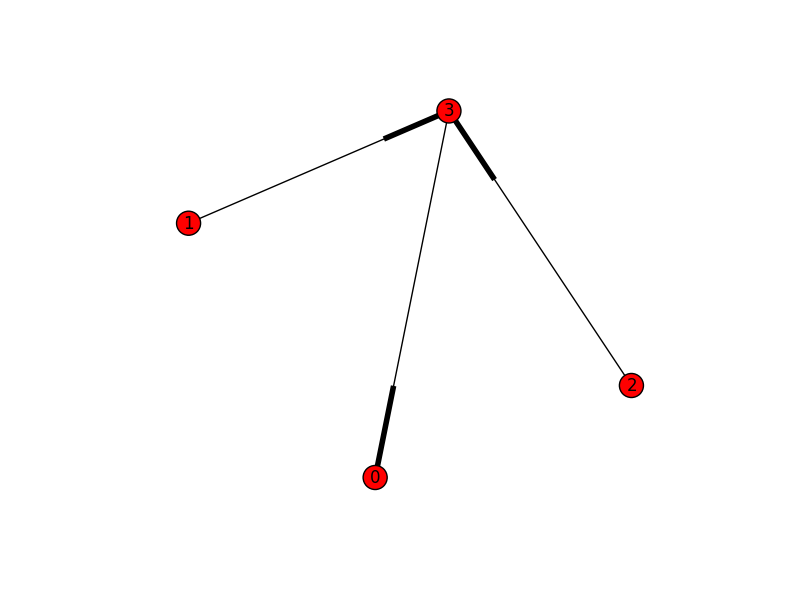
\includegraphics[scale=0.5]{./images/figure_1.PNG}\\
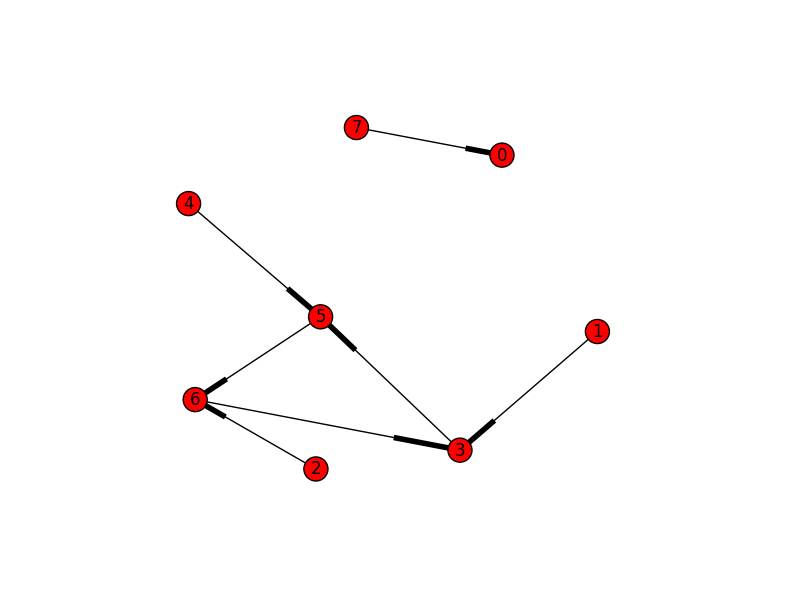
\includegraphics[scale=0.5]{./images/figure_2.PNG}
\end{center}
\caption{graphe de $A$ pour $n=2$ et $n=3$}
\end{figure}

%%%%%%%%%%%%%%%%%%%%%%%%%%%%%%%


\paragraph{\og Trafic automobile discret\fg{} :} l'ensemble $E$ contient des \og routes \fg{} toriques, c'est-\`a-dire des \'el\'ements correspondant aux \'ecritures en base $2$ sur $n$ bits d'entiers positifs : un $1$ repr\'esente une voiture et un $0$ repr\'esente un espace vide. Ainsi $E$ est de cardinal $2^n$. Pour $i\in [\![0,n-1]\!]$, on note $R_i$ l'$(i+1)$-\`eme bit de $R$ \`a partir de la droite. La fonction \'etudi\'ee ici est la suivante : 
\[\begin{aligned}f:\;&E\rightarrow E\\&R\mapsto R'\end{aligned}\]

o\`u

\[R'_{i}=\begin{cases}(\neg R_{i}\wedge R_{i+1})\vee(R_{i}\wedge R_{i-1}) &\text{si }0<i<n-1\\ (\neg R_{0}\wedge R_{1})\vee(R_{0}\wedge R_{n-1}) &\text{si }i=0\\ (\neg R_{n-1}\wedge R_{0})\vee(R_{n-1}\wedge R_{n-2}) &\text{si }i=n-1\end{cases}\text{ .}\]

Cette fonction n'est en fait que la formalisation du ph\'enom\`ene circulatoire concernant les routes de $E$ : \`a l'instant suivant une voiture peut se trouver \`a tel emplacement si et seulement si elle y est bloqu\'ee ou si elle n'\'etait pas bloqu\'ee \`a la position pr\'ec\'edente. Notons que les voitures se d\'eplacent de la gauche vers la droite.
\par